\RequirePackage{flashmovie}
\documentclass[compress]{beamer}%

\mode<presentation>
{
%	\setbeamertemplate{background canvas}[vertical shading][bottom=red!10,top=blue!10]
%	\usetheme{Frankfurt}
%    \usetheme{Berkeley}
%    \usetheme{Madrid}
    \usetheme{Warsaw}
%    \usetheme{JuanLesPins}
%    \usefonttheme[stillsansserifmath]{serif}
	\usefonttheme[onlymath]{serif}
    \usecolortheme{default}
}
%\setbeamercolor{background canvas}{bg=black}
%\usepackage{amsmath,amssymb,amsthm,mathrsfs,amsfonts,dsfont}
\usepackage{dsfont}
\usepackage{epstopdf}
\usepackage{multirow}
%\usepackage{epsfig}
\usepackage{amssymb}
\usepackage{amsmath}
\usepackage[absolute,overlay]{textpos}
\usepackage{keyval}
\usepackage{units}
\usepackage{geometry}
\usepackage{tabu}
\usepackage{multimedia}
%\usepackage{movie15}
\usepackage{hyperref}
\usepackage{graphics,graphicx,subfigure}
\usepackage{caption}

%\usepackage{subcaption}
%\newcommand{\myurlshort}[2]{\href{#1}{\textcolor{gray}{\textsf{#2}}}}%\usepackage{wrapfig}
%\usepackage{pst-all}
\usepackage{media9}%


\newtheorem*{mydef}{Definition}
\newtheorem*{mythm}{Theorem}
%
%%*******Define Mathematical operators***************
%%The number e
%\providecommand*{\eu}%
%            {\ensuremath{\mathrm{e}}}
%%For setting units
\providecommand*{\unit}[1]{%
	\ensuremath{\mathrm{\,#1}}}

%differentiation
\makeatletter
\providecommand*{\diff}%
    {\@ifnextchar^{\DIfF}{\DIfF^{}}}
\def\DIfF^#1{%
    \mathop{\mathrm{\mathstrut d}}%
        \nolimits^{#1}\gobblespace}
\def\gobblespace{%
    \futurelet\diffarg\opspace}
\def\opspace{%
    \let\DiffSpace\!%
    \ifx\diffarg(%
        \let\DiffSpace\relax
    \else
        \ifx\diffarg[%
            \let\DiffSpace\relax
    \else
        \ifx\diffarg\{%
            \let\DiffSpace\relax
        \fi\fi\fi\DiffSpace}

\providecommand*{\deriv}[3][]{%
    \frac{\diff^{#1}#2}{\diff #3^{#1}}}

\providecommand*{\pderiv}[3][]{%
\frac{\partial^{#1}#2}%
{\partial #3^{#1}}}

\DeclareMathOperator{\St}{St}
\DeclareMathOperator{\diag}{diag}
%%
%%%
%\usepackage{media9}%
%\newcommand{\includemovie}[3]{%
%\includemedia[%
%width=#1,height=#2,%
%activate=pagevisible,%
%deactivate=pageclose,%
%addresource=#3,%
%flashvars={%
%src=#3 % same path as in addresource!
%&autoPlay=true % default: false; if =true, automatically starts playback after activation (see option ‘activation)’
%&loop=true % if loop=true, media is played in a loop
%&controlBarAutoHideTimeout=0 %  time span before auto-hide
%}%
%]{}{myPresentation.avi}%
%

\newcommand*{\vcenteredhbox}[1]{\begingroup
\setbox0=\hbox{#1}\parbox{\wd0}{\box0}\endgroup}
\newcommand{\thepic}{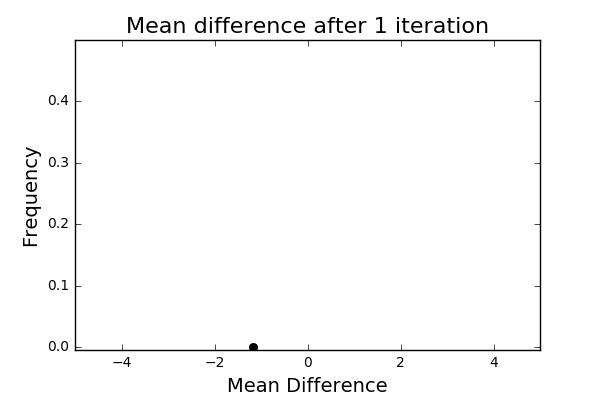
\includegraphics[width=5cm,height=5cm,keepaspectratio]{./figures/testp0.png}}

\begin{document}
\logo{
\includegraphics[height=.45cm,width=1.2cm]{./figures/uoftlogo.jpg}}
\title{Statistic Without Agonizing Pain
\hspace{2cm}}
\author{{Jamil Antoine Jabbour}}
\date{{December 17, 2016}}

\begin{frame}
\titlepage
\end{frame}
\setbeamercovered{transparent=10}

\begin{frame}
\frametitle{Motivation}
\begin{itemize}[<+->]
  \item Difficulty of understanding the assumptions and the fundamentals of statistical tests.
  \vspace{1cm}
  \item Most books/papers describe statistical  procedures without explanation of why or how they were invented.
  \vspace{1cm}
  \item Learning an elegant simple numerical method. 
\end{itemize}

\end{frame}


\begin{frame}
\frametitle{Thesis}
\vspace{-1cm}
\begin{center}
\alert{\Huge If you can program a computer, \\
then you have access to \\
the deepest and most\\
fundamental ideas\\ \vspace{.5cm}
in Statistics.}
\end{center}

\end{frame}

\begin{frame}
\centerline{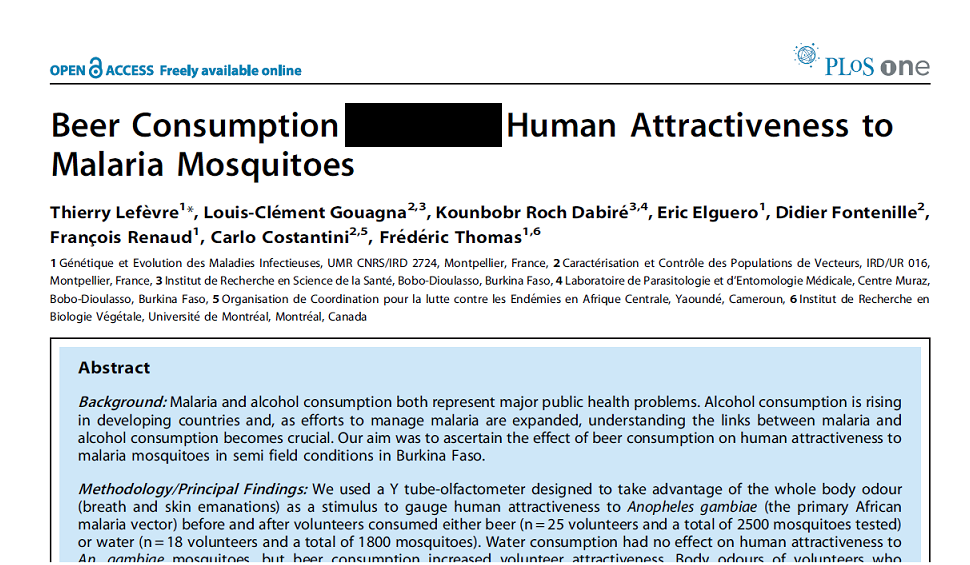
\includegraphics[height=7cm,width=12cm]{./figures/after.png}}
\end{frame}

\begin{frame}
\frametitle{Experiment}
\centerline{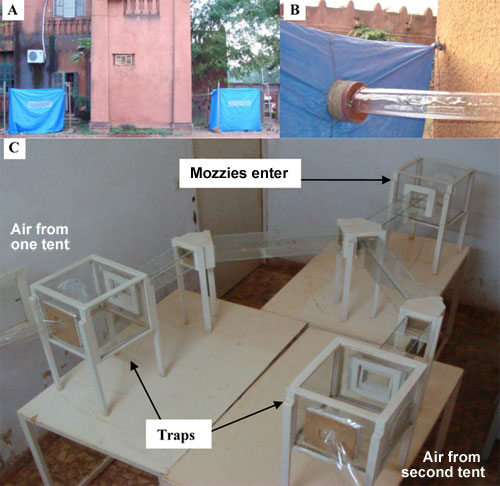
\includegraphics[height=6.5cm,width=11cm]{./figures/aparatus.jpg}}
\end{frame}

\begin{frame}[<+->]
\frametitle{Data}
\centerline{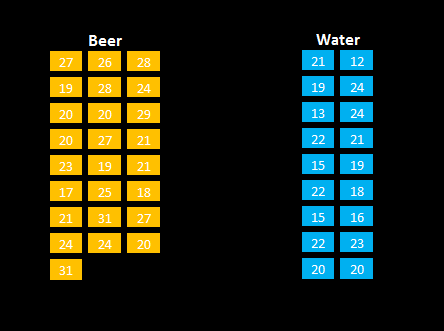
\includegraphics[height=5cm,width=9.5cm]{./figures/data.png}}
\begin{center}\begin{tabular}{ccccccccc}
 &&$\bar{X_b} = 23.6$ &&&& $\bar{X_w}= 19.2 $&&\\
 &&&&&&&& \\
&&&&  $\bar{X_b}- \bar{X_w} = 4.4$&&&&
\end{tabular}\end{center}
\end{frame}

\begin{frame}
\frametitle{Statistical Hypothesis}
\begin{enumerate}[<+->][A.]
  \item Beer consumption have no effect and the mean difference of~4.4 could have happened due to chance.
  \vspace{1.5cm}
  \item Compared to the sample variance in the sample, the mean difference of~4.4 is large and extremely unlikely to have happened due to  chance.
\end{enumerate}
\end{frame}

\begin{frame}
\frametitle{Approaches}
\begin{enumerate}[<+->]
  \item Analytical Approach (STAT 101)
  \vspace{2cm}
  \item Numerical  Approach
\end{enumerate}
\end{frame}

\begin{frame}
\frametitle{Statistical Analysis}
\centerline{BRING ON THE PAIN }
\centerline{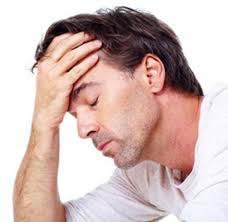
\includegraphics[height=5.5cm,width=11cm]{./figures/pain.jpg}}
\end{frame}

\begin{frame}
Welch's test, where we need to compute the t-statistics:
\begin{eqnarray*}
t_{stat} &=& \frac{\bar{X_1}-\bar{X_2}}{\sqrt{\frac{{s^2_1}}{n_1} +\frac{{s^2_2}}{n_2}}} \\
t_{stat} &=& \frac{23.6-19.2}{\sqrt{\frac{17.1}{25} +\frac{{13.5}}{18}}} \\
t_{stat} &=& 3.67.
\end{eqnarray*}
If the Statistical Hypothesis B is right then $t$ is distributed with this formula,
\begin{equation*}
  t(x,\nu) = \frac{\Gamma(\frac{\nu+1}{2})}{\sqrt{\nu\pi}\Gamma(\frac{\nu}{2})}\left(1 +\frac{x^2}{\nu} \right)^{-\frac{\nu+1}{2}},
\end{equation*}
\end{frame}

\begin{frame}
We need to estimate the degree of freedom then we use this formula,
\begin{eqnarray*}
\nu &\approx& \large \frac{\left(\frac{{s^2_1}}{n_1} +\frac{{s^2_2}}{n_2}\right)^2}{\left(\frac{s^2_1}{n_1}\right)^2\left(n_1 -1\right) + \left(\frac{{s^2_2}}{n_2}\right)^2\left(n_2 -1\right)}\\
\nu &\approx& \large \frac{\left(\frac{{4.1^2}}{25} +\frac{{3.1^2}}{18}\right)^2}{\left(\frac{4.1^2}{25}\right)^2\left(25 -1\right) + \left(\frac{{3.1^2}}{18}\right)^2\left(18 -1\right)}\\
~\\
\nu &\approx& 39.1.
\end{eqnarray*}
\end{frame}

\begin{frame}
\frametitle{Analysis Results}
\begin{center}
\vspace{-1.5cm}\begin{tabular}{p{4.5cm}p{.5cm}c}
  \small Obtaining the $t_c$ from $t$-table and comparing it to $t_{stat}$:
  &&\multirow{4}{*}{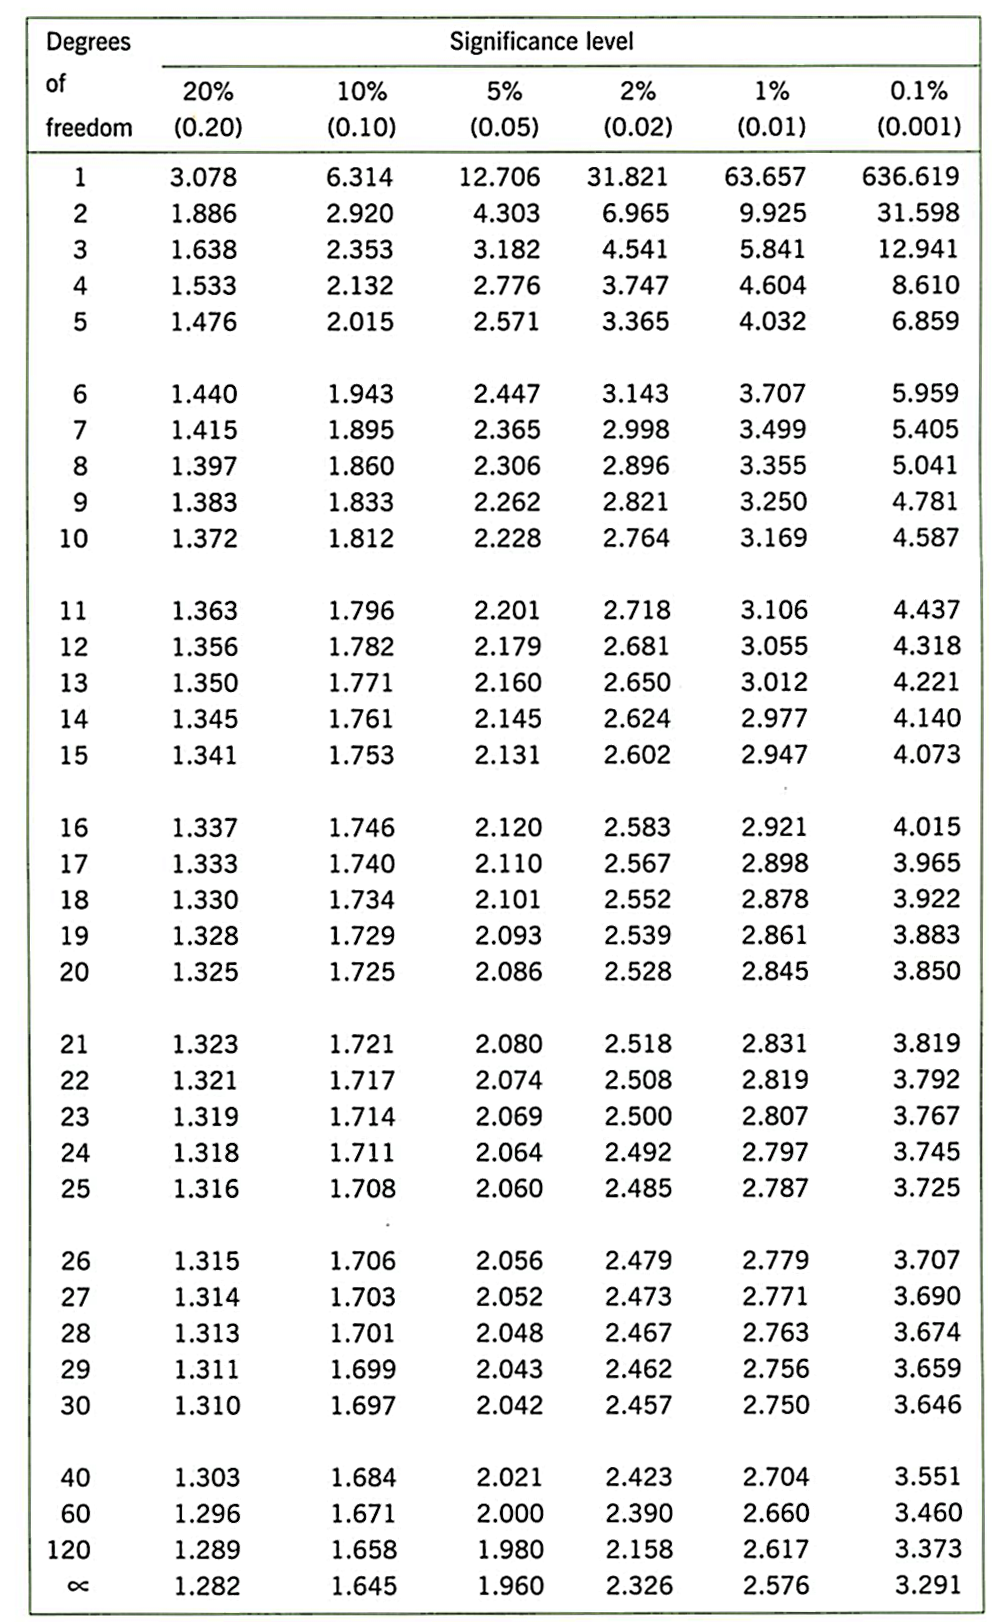
\includegraphics[height=7cm]{./figures/ttable.png}} \\
  $t_c = 2.021 < 3.67 = t_{stat}$ && \\
  \vspace{1cm} Therefore, 4.4 difference of additional mosquitoes is statistically significant at (p~=~0.05) &&
\end{tabular}\end{center}
\end{frame}

\begin{frame}
\frametitle{Numerical Approach}
\vspace{-1.5cm}
In the case of  Hypothesis A, the data can be considered as labels.
\begin{center}
  \begin{tabular}{p{5cm}c}
    1. Shuffle the data randomly  & \multirow{7}{*}{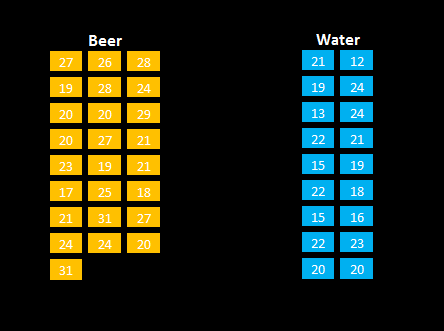
\includegraphics[height=5cm,width=6cm]{./figures/data.png}} \\
    &\\
    2. Compute mean difference& \\
    &\\
    3. Store mean difference & \\
    &\\
    4. Repeat (1,2,3)
  \end{tabular}
\end{center}
\end{frame}

\begin{frame}
 \vcenteredhbox{{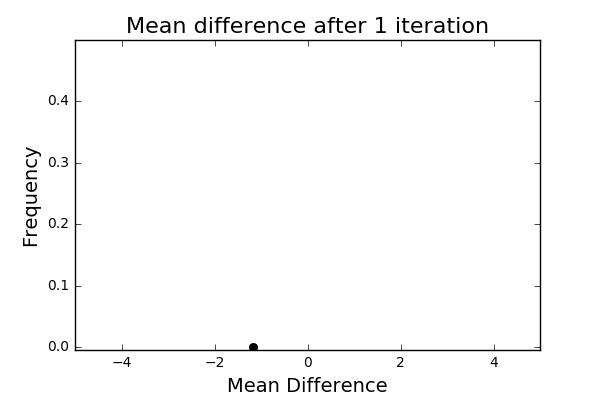
\includegraphics[width=5cm,height=5cm,keepaspectratio]{./figures/testp0.png}}}
 \vcenteredhbox{\alt<2->{{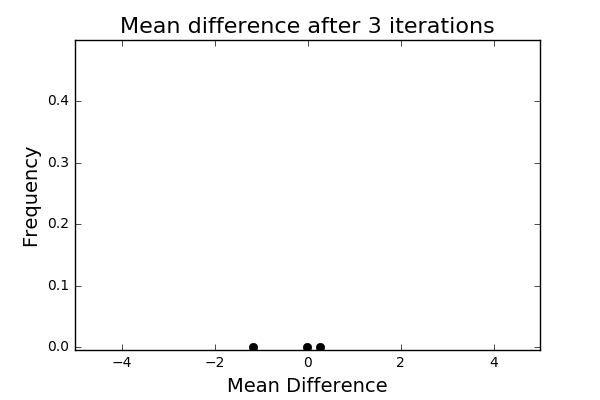
\includegraphics[width=5cm,height=5cm,keepaspectratio]{./figures/testp1.png}}}{\phantom{\thepic}}}
 \vcenteredhbox{\alt<3->{{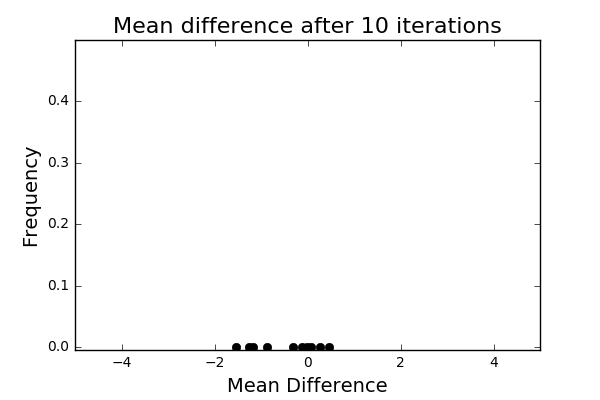
\includegraphics[width=5cm,height=5cm,keepaspectratio]{./figures/testp2.png}}}{\phantom{\thepic}}}
 \vcenteredhbox{\alt<4->{{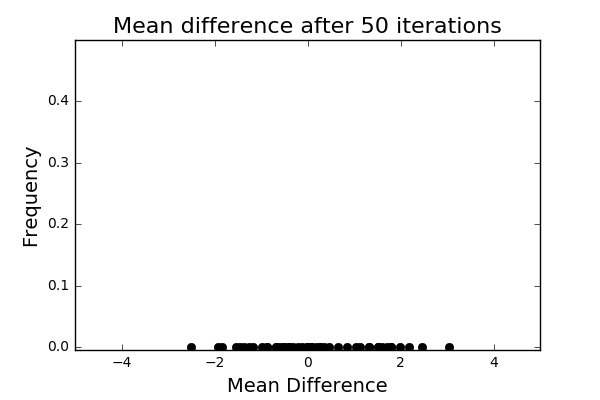
\includegraphics[width=5cm,height=5cm,keepaspectratio]{./figures/testp3.png}}}{\phantom{\thepic}}}
\end{frame}

\begin{frame}
\centerline{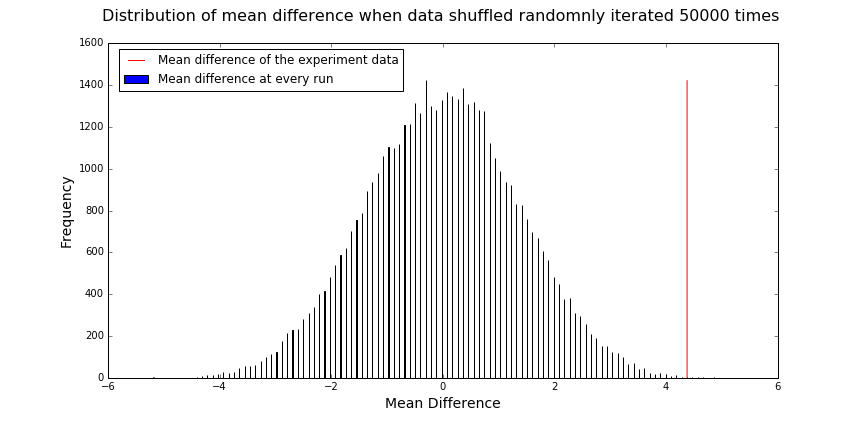
\includegraphics[height=7cm,width=12cm]{./figures/distribution_50k.png}}
\end{frame}


\begin{frame}
\centerline{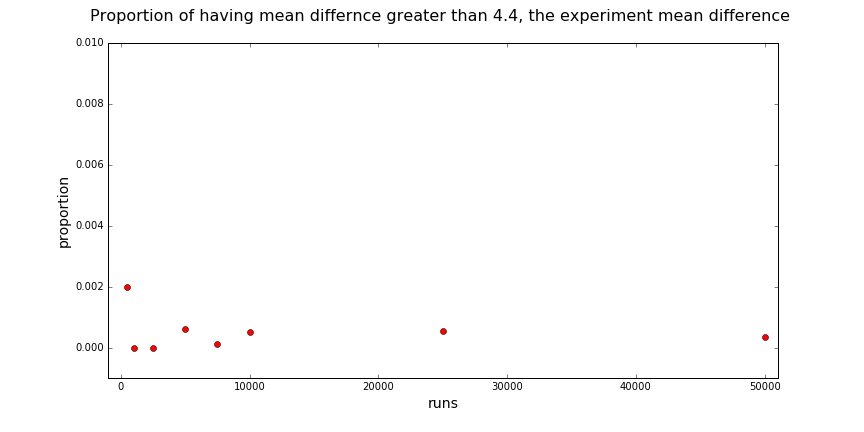
\includegraphics[height=7cm,width=12cm]{./figures/proportion.png}}
\end{frame}

\begin{frame}
\centerline{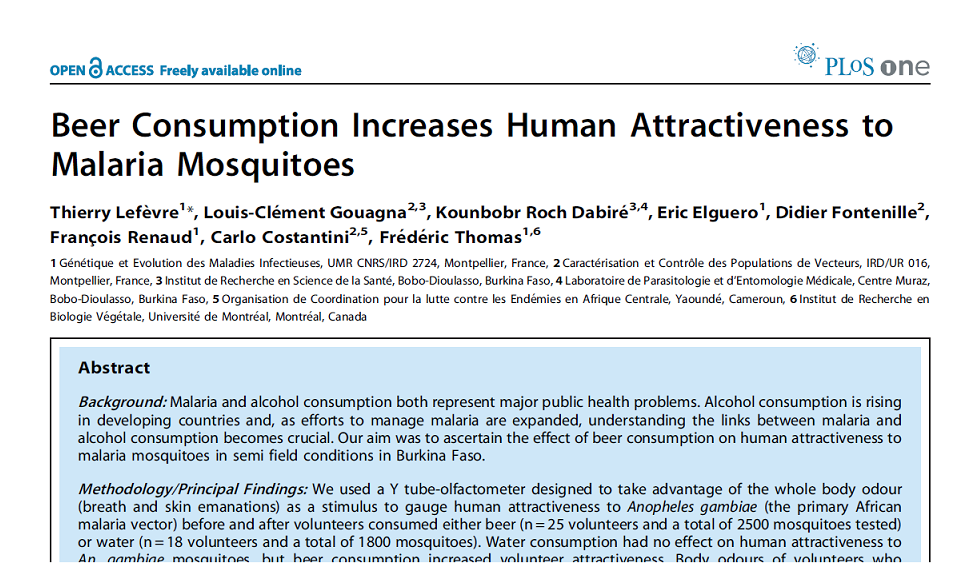
\includegraphics[height=7cm,width=12cm]{./figures/before.png}}
\end{frame}

\begin{frame}
\frametitle{Conclusion}
\begin{enumerate}
  \item Ability to follow a simple logical argument.
  \vspace{1cm}
  \item Ability to generate random number.
  \vspace{1cm}
  \item Ability to repeat the process i.e. iteration.
\end{enumerate}
\end{frame}


\end{document} 